\subsection{Physikalische Grundlagen}
\label{sec:physikalisches_prinzip}

Physikalisch betrachtet basiert die Funktionsweise des Messstromwandlers auf dem Wirkprinzip eines kurzgeschlossenen Transformators~\cite[S.~63]{book-Technologie_Messwandler-Minkner}. Die Wandlung beruht auf der elektromagnetischen Kopplung zwischen dem Primärleiter und der Sekundärwicklung über einen Magnetkern~\cite[S.~63]{book-Technologie_Messwandler-Minkner}. Zur Analyse des Betriebsverhaltens sowie potenzieller Fehlerquellen werden im Folgenden die theoretischen Zusammenhänge der magnetischen Induktion hergeleitet~\cite[Kap.~11]{book-Magnetisches_Feld_Moeller-Harriehausen}.



Die Betrachtung beginnt bei der Entstehung der magnetischen Feldstärke \gls{sym:H} durch den Primärstrom \gls{sym:I_p} und führt unter Berücksichtigung der Materialeigenschaften des Kerns zur magnetischen Flussdichte \gls{sym:B}~\cite[Kap.~4.5.4]{book-Physik_Ingenieure-Hering}. Unter Einbeziehung der geometrischen Abmessungen wird der magnetische Widerstand \gls{sym:Rm} definiert, welcher die Grundlage für das Hopkinsonsche Gesetz bildet~\cite[Kap.~11.9]{book-Magnetisches_Feld_Moeller-Harriehausen}. Abschließend wird erläutert, wie sich durch die induzierte Gegendurchflutung auf der Sekundärseite das für die Stromtransformation erforderliche Durchflutungsgleichgewicht \gls{sym:Theta} einstellt~\cite[S.~75]{book-Technologie_Messwandler-Minkner}.

\subsubsection{Magnetfelder und Induktion}
\label{sec:physik_grundlagen_induktion}

Die physikalische Grundlage eines Stromwandlers bildet die elektromagnetische Kopplung zwischen dem Primärleiter und dem Sekundärkreis über einen magnetischen Kern. Dieser Zusammenhang wird durch die Maxwell-Gleichungen~\cite[Kap.~4.5.4]{book-Physik_Ingenieure-Hering} beschrieben und lässt sich idealisiert am Modell des magnetischen Kreises herleiten, wie in Abbildung~\ref{pic:phy_wandler} schematisch dargestellt ist.

\begin{figure}[H]
    \centering
    \includegraphics[width=0.8\textwidth]{03_Ressourcen/zeichnungen/phy_wandler.drawio.pdf}
    \caption{Schematische Darstellung der magnetischen Kopplung im Wandler}
    \label{pic:phy_wandler}
\end{figure}

Ein durch den Ringkern geführter Primärstrom \gls{sym:I_p} erzeugt gemäß dem Ampèreschen Durchflutungsgesetz ein magnetisches Feld~\cite[Kap.~4.5.4]{book-Physik_Ingenieure-Hering}. Das Linienintegral der magnetischen Feldstärke \gls{sym:H} entlang eines geschlossenen Weges $\mathcal{S}$ entspricht dabei der umschlossenen Durchflutung \gls{sym:Theta}, wie Gleichung \eqref{eq:ampere_integral} verdeutlicht~\cite[Kap.~4.5.4]{book-Physik_Ingenieure-Hering}:

\begin{equation}
    \oint_{\mathcal{S}} \vec{H}\cdot d\vec{s} = \Theta = N_p \cdot I_p
    \label{eq:ampere_integral}
\end{equation}

Der Stromwandler nutzt einen Ringkern aus ferromagnetischem Material mit einer hohen relativen Permeabilität \gls{sym:mur} $\gg \num{1,00}$ (siehe Abschnitt \ref{sec:magnetische_stoffeigenschaften})~\cite[Tab.~48]{book-Taschenbuch_Physik-Kuchling}. Unter der Annahme eines torusförmigen Kerns mit dem mittleren Radius \gls{sym:r} folgt der Integrationsweg der kreisförmigen mittleren Feldlinie. Infolge der Rotationssymmetrie bleibt der Betrag der Feldstärke \gls{sym:H} konstant. Bei einem Durchsteck- oder Aufsteckstromwandler entspricht der Primärleiter physikalisch einer einzelnen Windung, sodass für die primäre Windungszahl \gls{sym:Np} = \num{1,00} gilt~\cite[S.~63]{book-Technologie_Messwandler-Minkner}. Das Wegintegral ergibt sich folglich aus dem Produkt der Feldstärke \gls{sym:H} und dem Kreisumfang $2\pi r$ (siehe Gleichung \eqref{eq:feldstaerke_h})~\cite[Kap.~4.5.4]{book-Physik_Ingenieure-Hering}.

\begin{align}
    \oint_{\mathcal{S}} \vec{H} \cdot \mathrm{d}\vec{s} & = H \cdot \oint_{\mathcal{S}} \mathrm{d}s = H \cdot 2\pi r = I_{p} \nonumber \\[6pt]
    \Rightarrow \quad H                                 & = \frac{I_{p}}{2\pi r}
    \label{eq:feldstaerke_h}
\end{align}

Die magnetische Flussdichte \gls{sym:B} im Kernmaterial resultiert aus der Feldstärke und den materialspezifischen Eigenschaften. Mit der magnetischen Feldkonstante \gls{sym:mu0} und der relativen Permeabilität \gls{sym:mur} folgt der Zusammenhang in Gleichung \eqref{eq:flussdichte_b}~\cite[Kap.~4.5.4]{book-Physik_Ingenieure-Hering}:

\begin{equation}
    B = \mu_0 \mu_r \cdot H = \mu_0 \mu_r \cdot \frac{I_{p}}{2\pi r}
    \label{eq:flussdichte_b}
\end{equation}

Für die Funktion des Stromwandlers ist entscheidend, welcher magnetische Fluss \gls{sym:Phi} den Eisenquerschnitt \gls{sym:A} durchsetzt, da dieser in der Sekundärwicklung die Spannung induziert~\cite[S.~67]{book-Technologie_Messwandler-Minkner}. Der Fluss berechnet sich durch die Integration der Flussdichte über die Querschnittsfläche gemäß Gleichung \eqref{eq:fluss_integral}~\cite[Kap.~4.5.4]{book-Physik_Ingenieure-Hering}:

\begin{equation}
    \Phi = \iint_A \vec{B} \cdot \mathrm{d}\vec{A}
    \label{eq:fluss_integral}
\end{equation}



Unter der Annahme einer über den Querschnitt konstanten Flussdichte ($\vec{B} \parallel \mathrm{d}\vec{A}$) ergibt sich der direkte Zusammenhang zwischen dem verursachenden Primärstrom und dem resultierenden magnetischen Fluss im Kern (siehe Gleichung \eqref{eq:fluss_final})~\cite[Kap.~4.5.4]{book-Physik_Ingenieure-Hering}:

\begin{equation}
    \Phi = B \cdot A = \mu_0 \mu_r \frac{A}{2\pi r} \cdot I_{p}
    \label{eq:fluss_final}
\end{equation}

Dieser Ausdruck zeigt, dass der magnetische Fluss im Wandlerkern – unter Ausschluss von Sättigungseffekten – proportional zum Primärstrom \gls{sym:I_p} ist~\cite[Kap.~11]{book-Magnetisches_Feld_Moeller-Harriehausen}. Der Faktor $\mu_0 \mu_r \frac{A}{2\pi r}$ fasst dabei die Geometrie (Querschnitt \gls{sym:A} und Umfang $2\pi r$) sowie die magnetischen Eigenschaften des Kerns zusammen.

Der hergeleitete Zusammenhang lässt sich in Analogie zum elektrischen Stromkreis (Ohmsches Gesetz) betrachten. Der Term, welcher die Geometrie und Materialeigenschaften beschreibt, definiert den magnetischen Widerstand \gls{sym:Rm} (siehe Gleichung \eqref{eq:magnetischer_widerstand})~\cite[Kap.~11.9]{book-Magnetisches_Feld_Moeller-Harriehausen}:

\begin{equation}
    R_m = \frac{2\pi r}{\mu_0 \mu_r A}
    \label{eq:magnetischer_widerstand}
\end{equation}

Damit lässt sich der magnetische Fluss \gls{sym:Phi} über das Hopkinsonsche Gesetz ausdrücken, welches das magnetische Äquivalent zum Ohmschen Gesetz bildet. Die magnetische Durchflutung \gls{sym:Theta} entspricht dabei der elektrischen Spannung und der magnetische Fluss dem elektrischen Strom (vgl. Gleichung \eqref{eq:hopkinson}) \cite[Kap.~11.9]{book-Magnetisches_Feld_Moeller-Harriehausen}:

\begin{equation}
    \Phi = \frac{\Theta}{R_m}
    \label{eq:hopkinson}
\end{equation}

Im Betrieb des Stromwandlers wirkt nicht nur der Primärstrom auf den magnetischen Kreis. Auf der Sekundärseite befindet sich eine Wicklung mit der Windungszahl \gls{sym:Ns}. Der magnetische Fluss induziert in dieser Wicklung eine Spannung, die bei geschlossenem Sekundärkreis einen Sekundärstrom \gls{sym:I_sec} treibt~\cite[S.~67]{book-Technologie_Messwandler-Minkner}. Nach der Lenzschen Regel wirkt dieser Sekundärstrom seiner Ursache entgegen~\cite[S.~20]{pdf-Skript_Induktion-Rolink}. Er erzeugt eine magnetische Gegendurchflutung $\Theta_{s}$, welche den Fluss im Kern schwächt. Die resultierende magnetische Durchflutung $\Theta_{res}$, die effektiv den Fluss im Kern treibt, ist somit die Differenz aus Primär- und Sekundärdurchflutung (siehe Gleichung \eqref{eq:durchflutungsbilanz})~\cite[S.~75]{book-Technologie_Messwandler-Minkner}:

\begin{equation}
    \Theta_{res} = \Theta_{p} - \Theta_{s} = N_{p} \cdot I_{p} - N_{s} \cdot I_{s}
    \label{eq:durchflutungsbilanz}
\end{equation}

Setzt man die resultierende Durchflutung in das Hopkinsonsche Gesetz ein, erhält man die Beziehung in Gleichung \eqref{eq:bilanz_rm}~\cite[Kap.~11.9]{book-Magnetisches_Feld_Moeller-Harriehausen}:

\begin{equation}
    \Phi \cdot R_m = N_{p} \cdot I_{p} - N_{s} \cdot I_{s}
    \label{eq:bilanz_rm}
\end{equation}

Für die ideale Betrachtung eines Stromwandlers wird ein Kernmaterial mit unendlich hoher Permeabilität ($\mu_r \to \infty$) angenommen~\cite[Kap.~11]{book-Magnetisches_Feld_Moeller-Harriehausen}. Daraus folgt gemäß Gleichung \eqref{eq:magnetischer_widerstand}, dass der magnetische Widerstand gegen \num{0,00} strebt ($R_m \to 0,00$). Damit der magnetische Fluss \gls{sym:Phi} einen endlichen Wert annimmt, muss die resultierende Durchflutung ebenfalls gegen \num{0,00} streben. Es stellt sich ein nahezu ideales Durchflutungsgleichgewicht ein (siehe Gleichung \eqref{eq:ideales_gleichgewicht})~\cite[S.~75]{book-Technologie_Messwandler-Minkner}:

\begin{align}
    0                         & = N_{p} \cdot I_{p} - N_{s} \cdot I_{s} \nonumber \\[6pt]
    N_{s} \cdot I_{s} & = N_{p} \cdot I_{p}
    \label{eq:ideales_gleichgewicht}
\end{align}

Durch Umstellen dieser Gleichung ergibt sich der Sekundärstrom \gls{sym:I_sec} in Abhängigkeit vom Primärstrom \gls{sym:I_p} und dem Übersetzungsverhältnis der Windungszahlen (siehe Gleichung \eqref{eq:sekundaerstrom})~\cite[S.~63]{book-Technologie_Messwandler-Minkner}:

\begin{equation}
    I_{s} = I_{p} \cdot \frac{N_{p}}{N_{s}}
    \label{eq:sekundaerstrom}
\end{equation}

Diese Beziehung beschreibt das ideale Übertragungsverhalten des Stromwandlers, bei dem der Sekundärstrom proportional zum Primärstrom ist und lediglich durch das Windungszahlverhältnis skaliert wird~\cite[S.~63]{book-Technologie_Messwandler-Minkner}.


\subsubsection{Magnetische Stoffeigenschaften}
\label{sec:magnetische_stoffeigenschaften}

Magnetische Stoffeigenschaften charakterisieren die Reaktion eines Materials auf ein externes Magnetfeld~\cite[Kap.~11]{book-Magnetisches_Feld_Moeller-Harriehausen}. Als zentrale Kenngröße dient die relative Permeabilität \gls{sym:mur}, welche die magnetische Flussdichte \gls{sym:B} im Material ins Verhältnis zur Flussdichte im Vakuum setzt~\cite[Tab.~48]{book-Taschenbuch_Physik-Kuchling}. Tabelle~\ref{tab:magnetische_stoffeigenschaften} gibt eine systematische Einteilung der magnetischen Stoffklassen sowie typische Wertebereiche der Permeabilität \gls{sym:mur} nach \cite[Tab.~48]{book-Taschenbuch_Physik-Kuchling} wieder.

\begin{table}[H]
    \centering
    \caption{Magnetische Stoffklassen und typische Bereiche der relativen Permeabilität \gls{sym:mur} nach \cite[Tab.~48]{book-Taschenbuch_Physik-Kuchling}}
    \label{tab:magnetische_stoffeigenschaften}
    \begin{tabular}{lccc}
        \toprule
        \textbf{Eigenschaft} & \textbf{Permeabilität \gls{sym:mur}} & \textbf{Verhalten}        & \textbf{Materialien}   \\ 
        \midrule
        Diamagnetismus       & $< \num{1,00}$                       & Feldschwächung            & Bi, Cu, Ag, Au, $\text{H}_2\text{O}$ \\
        Paramagnetismus      & $> \num{1,00}$                       & Schwache Verstärkung      & Al, Pt, Mg, Luft       \\
        Ferromagnetismus     & $\gg \num{1,00}$                     & Starke Verstärkung        & Fe, Co, Ni, Mu-Metall  \\
        Ferrimagnetismus     & $\gg \num{1,00}$                     & Permanente Magnetisierung & Ferrite, Magnetit      \\
        Antiferromagnetismus & $\approx \num{1,00}$                 & Keine äußere Wirkung      & Mn, Cr, MnO            \\
        \bottomrule
    \end{tabular}
\end{table}

Diamagnetische Stoffe weisen eine relative Permeabilität \gls{sym:mur} kleiner als \num{1,00} auf, wie beispielsweise Kupfer oder Wasser~\cite[Tab.~48]{book-Taschenbuch_Physik-Kuchling}. Paramagnetische und diamagnetische Materialien werden in vielen elektrotechnischen Anwendungen näherungsweise als vakuumähnlich behandelt, da ihre Abweichung von $\mu_r \approx \num{1,00}$ geringfügig ist~\cite[Tab.~48]{book-Taschenbuch_Physik-Kuchling}. Für Messstromwandler sind hingegen ferromagnetische Werkstoffe essenziell, da deren hohe Permeabilität \gls{sym:mur} den magnetischen Fluss \gls{sym:Phi} konzentriert im Kern führt und somit eine effiziente induktive Kopplung ermöglicht~\cite[S.~63]{book-Technologie_Messwandler-Minkner}.

Da die Permeabilität ferromagnetischer Materialien nichtlinear von der Feldstärke \gls{sym:H} abhängt, tritt bei hohen Feldstärken die magnetische Sättigung ein~\cite[Kap.~11]{book-Magnetisches_Feld_Moeller-Harriehausen}. In diesem Zustand nimmt die wirksame Permeabilität \gls{sym:mur} signifikant ab, wodurch die Übertragungsgenauigkeit bei hohen Primärströmen \gls{sym:I_p} oder unter externem Fremdfeldeinfluss abfällt~\cite[S.~73]{book-Technologie_Messwandler-Minkner}.

\subsubsection{Hysterese und reales Verhalten}
\label{sec:hysterese-und-reales_verhalten}

Ferromagnetische Werkstoffe zeichnen sich durch eine nichtlineare Magnetisierungskennlinie aus, deren physikalische Ursache in der Domänenstruktur des Materials begründet liegt~\cite[Kap.~11]{book-Magnetisches_Feld_Moeller-Harriehausen}. Im Kristallgefüge bilden sich mikroskopische Bereiche, die als magnetische Domänen oder \textit{Weißsche Bezirke} bezeichnet werden~\cite[Kap.~11]{book-Magnetisches_Feld_Moeller-Harriehausen}. Innerhalb dieser Domänen sind die atomaren magnetischen Momente parallel orientiert, woraus eine lokale Sättigungsmagnetisierung resultiert~\cite[Kap.~11]{book-Magnetisches_Feld_Moeller-Harriehausen}. Die räumlich begrenzten Übergangszonen zwischen benachbarten Domänen mit unterschiedlicher Magnetisierungsrichtung werden als Bloch-Wände bezeichnet~\cite[Kap.~11]{book-Magnetisches_Feld_Moeller-Harriehausen}.



Abbildung~\ref{fig:weiss_bezirke} illustriert die Veränderung dieser Domänenstruktur unter Einwirkung eines äußeren Magnetfeldes. Im unmagnetisierten Ausgangszustand ist die Domänenverteilung statistisch so angeordnet, dass die resultierende Magnetisierung nach außen näherungsweise \num{0,00} beträgt~\cite[Kap.~11]{book-Magnetisches_Feld_Moeller-Harriehausen}.

\begin{figure}[H]
    \centering
    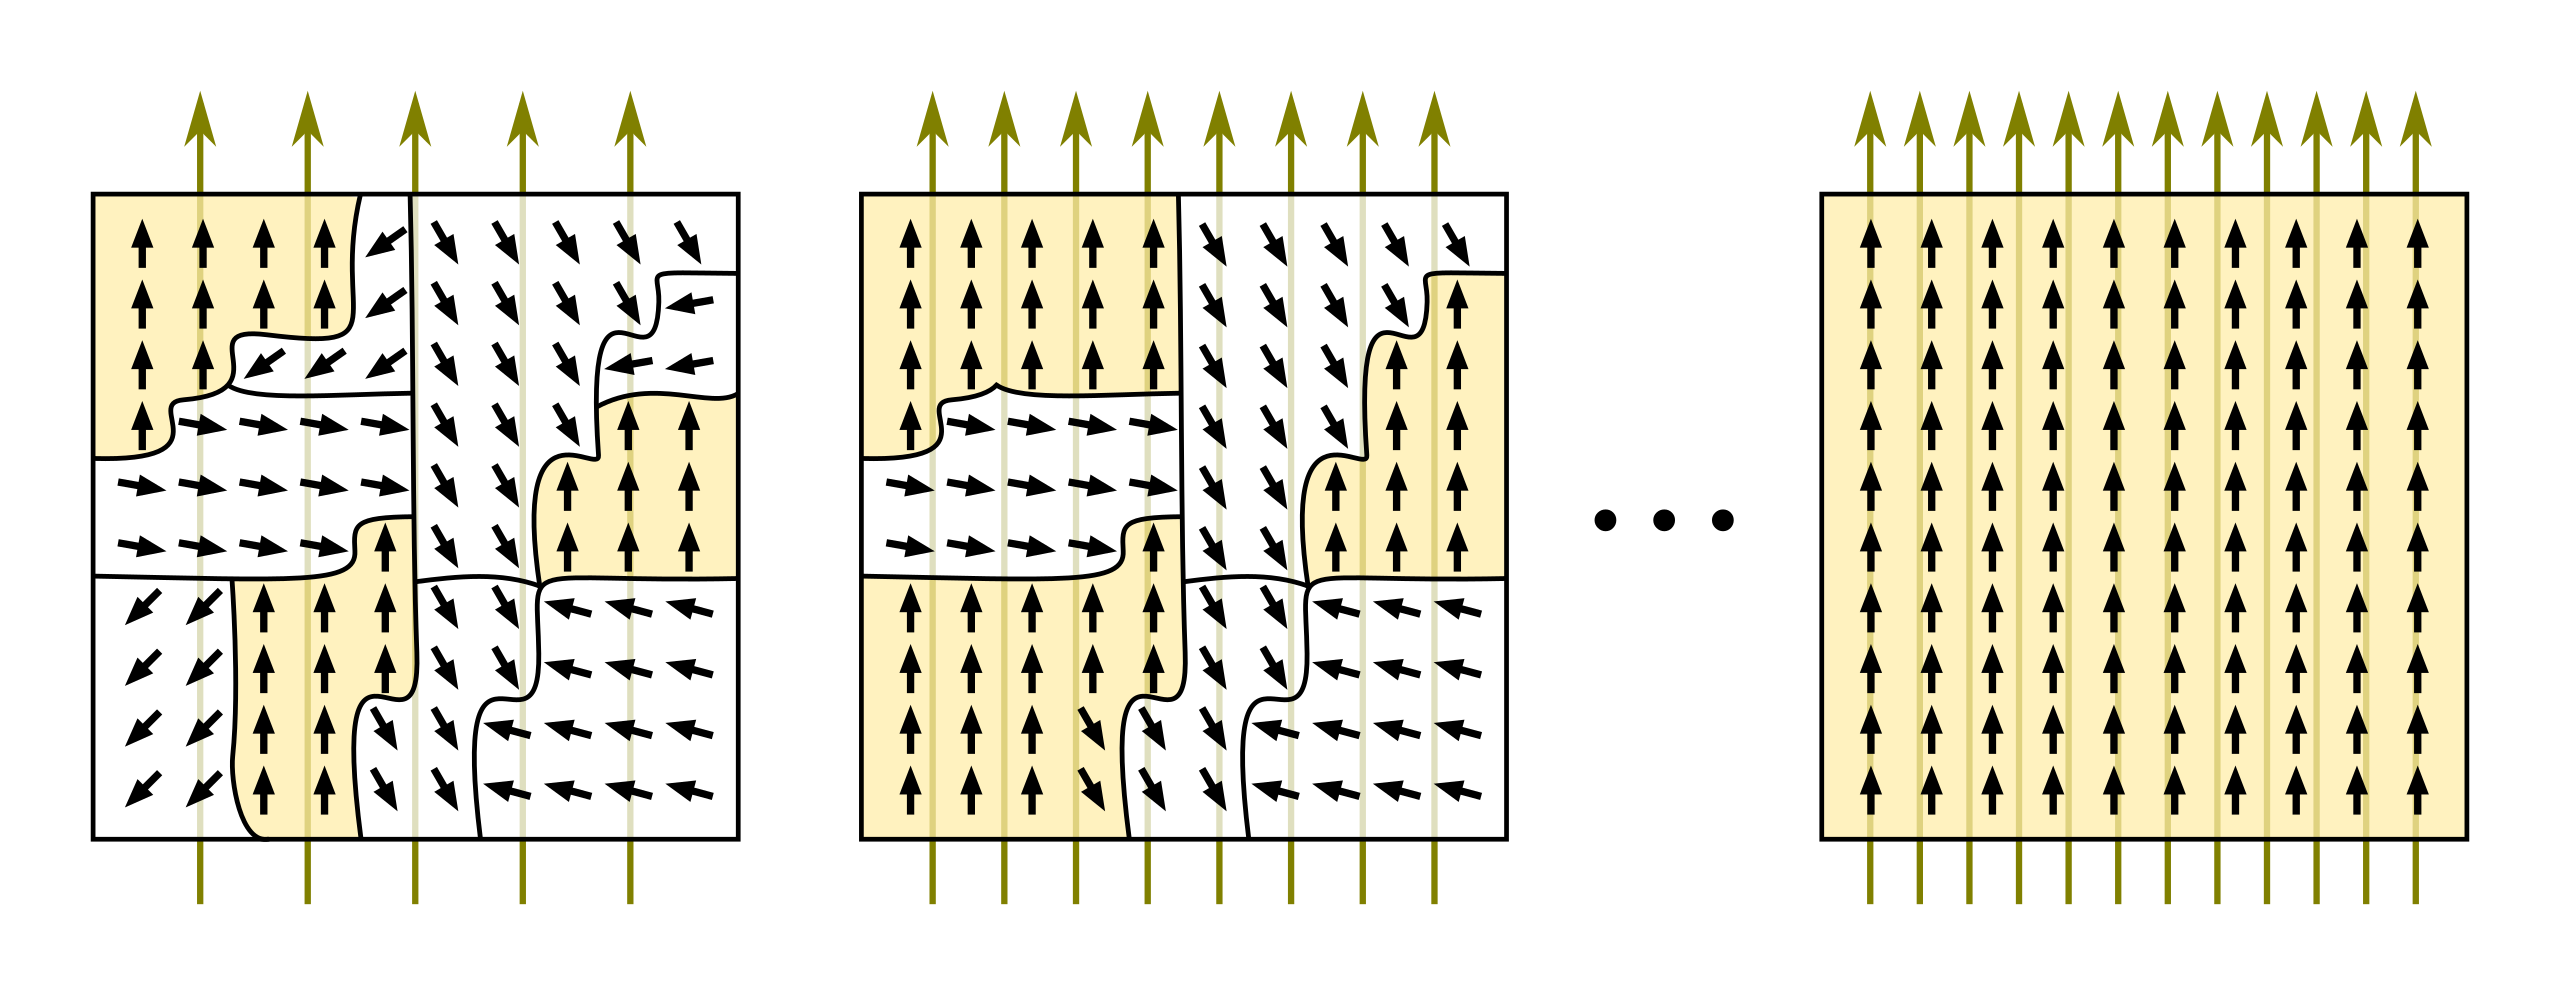
\includegraphics[width=0.8\textwidth]{03_Ressourcen/Bilder/growing-magnetic-domains.svg.png}
    \caption{Schematische Darstellung der Domänenentwicklung bei Anlegen eines äußeren Magnetfeldes, nach \cite{image-Growing_magnetic_domains-MikeRun}}
    \label{fig:weiss_bezirke}
\end{figure}

Mit steigender Feldstärke \gls{sym:H} wachsen energetisch günstig orientierte Domänen an~\cite[Kap.~11]{book-Magnetisches_Feld_Moeller-Harriehausen}. Dieser Prozess erfolgt initial primär durch die Verschiebung der Bloch-Wände~\cite[Kap.~11]{book-Magnetisches_Feld_Moeller-Harriehausen}. Bei einer weiteren Erhöhung der Feldstärke setzt die Drehung der magnetischen Momente innerhalb der Domänen ein, bis eine vollständige Ausrichtung in Feldrichtung erreicht ist~\cite[Kap.~11]{book-Magnetisches_Feld_Moeller-Harriehausen}. Dieser Endzustand definiert die magnetische Sättigung~\cite[Kap.~11]{book-Magnetisches_Feld_Moeller-Harriehausen}. In diesem Bereich führt eine weitere Steigerung der Feldstärke \gls{sym:H} nur noch zu einer marginalen Erhöhung der Flussdichte \gls{sym:B}, da die maximale Magnetisierung des Materials erreicht ist~\cite[Kap.~11]{book-Magnetisches_Feld_Moeller-Harriehausen}.

Diese nichtlineare Domänenumordnung bewirkt, dass die effektive Permeabilität \gls{sym:mur} im Sättigungsbereich drastisch sinkt~\cite[Kap.~11]{book-Magnetisches_Feld_Moeller-Harriehausen}. Für Messstromwandler resultiert daraus eine reduzierte Messgenauigkeit bei hohen Primärströmen \gls{sym:I_p} oder bei überlagerten magnetischen Fremdfeldern~\cite[S.~73]{book-Technologie_Messwandler-Minkner}.

Zusätzlich zur Nichtlinearität tritt das Phänomen der Hysterese auf. Dies beschreibt den Umstand, dass die Flussdichte \gls{sym:B} bei veränderlicher Feldstärke \gls{sym:H} nicht nur vom aktuellen Wert, sondern vom vorherigen Magnetisierungszustand abhängt~\cite[Kap.~11]{book-Magnetisches_Feld_Moeller-Harriehausen}. Abbildung~\ref{fig:bh-hysterese} verdeutlicht dieses Verhalten im $B$-$H$-Diagramm.

% [Image of magnetic hysteresis curve]

Die Neukurve beschreibt den initialen Magnetisierungsvorgang eines unmagnetisierten Materials bis zur Sättigung~\cite[Kap.~11]{book-Magnetisches_Feld_Moeller-Harriehausen}. Bei anschließender Reduktion der Feldstärke \gls{sym:H} verläuft die Flussdichte \gls{sym:B} entlang einer Hystereseschleife und kehrt nicht zum Nullpunkt zurück~\cite[Kap.~11]{book-Magnetisches_Feld_Moeller-Harriehausen}. Ursächlich hierfür sind irreversible Verschiebungen der Bloch-Wände, die durch Gitterdefekte im Kristallgefüge behindert werden~\cite[Kap.~11]{book-Magnetisches_Feld_Moeller-Harriehausen}. Bei einer Feldstärke von \gls{sym:H} = \num{0,00} verbleibt die Remanenzflussdichte \gls{sym:Br}~\cite[Kap.~11]{book-Magnetisches_Feld_Moeller-Harriehausen}. Zur vollständigen Entmagnetisierung muss eine Gegenfeldstärke aufgebracht werden, deren Betrag als Koerzitivfeldstärke \gls{sym:Hc} definiert ist~\cite[Kap.~11]{book-Magnetisches_Feld_Moeller-Harriehausen}.

\begin{figure}[H]
    \centering
    \includegraphics[width=0.8\textwidth]{03_Ressourcen/simulation/hysterese/hysterese_kurve_final_colors.pdf}
    \caption{Schematische Darstellung von Neukurve und Hystereseschleife im $B$-$H$-Diagramm}
    \label{fig:bh-hysterese}
\end{figure}

Die von der Hystereseschleife umschlossene Fläche korreliert direkt mit den magnetischen Umagnetisierungsverlusten pro Zyklus~\cite[Kap.~11.12.1]{book-Magnetisches_Feld_Moeller-Harriehausen}. In der Messtechnik werden daher bevorzugt weichmagnetische Werkstoffe mit geringer Koerzitivfeldstärke \gls{sym:Hc} und schmaler Hystereseschleife eingesetzt, um die Remanenz \gls{sym:Br} sowie die Verlustleistung zu minimieren~\cite{book-Magnetisches_Feld_Moeller-Harriehausen, website-Magnetisierungskurve-Mietke}.



\subsubsection{Störeinflüsse bei Messstromwandlern}
\label{sec:stoerfelder_schaltanlagen}

Die Genauigkeit von Messstromwandlern im Betrieb wird maßgeblich von externen und systembedingten Faktoren beeinflusst~\cite[S.~65]{book-Technologie_Messwandler-Minkner}. Die wesentlichen Störeinflüsse gliedern sich in die drei Kategorien fehlerhafte Bürdenbeschaltung, Einwirkung externer magnetischer Fremdfelder sowie geometrische Positionierung des Primärleiters~\cite[S.~65]{book-Technologie_Messwandler-Minkner}.

% --- Paragraph 1 ---
\paragraph{Einfluss der Bürde}
\label{par:einfluss_buerde}

Die Impedanz der Bürde bestimmt das Betriebsverhalten des Stromwandlers maßgeblich~\cite[S.~65]{book-Technologie_Messwandler-Minkner}.
Wie im vereinfachten Ersatzschaltbild (Abbildung~\ref{esb:wandler_vereinfacht}) dargestellt, setzt sich der Sekundärkreis aus der Innenimpedanz der Wicklung und der externen Bürde zusammen~\cite[S.~65]{book-Technologie_Messwandler-Minkner}.
Ein erhöhter Widerstand im Sekundärkreis erfordert eine höhere induzierte Spannung $U_o$ zur Aufrechterhaltung des eingeprägten Stroms $I_s$~\cite[S.~67]{book-Technologie_Messwandler-Minkner}.
Diese Spannung entspricht der Summe der Spannungsabfälle über dem Wicklungswiderstand $R_s$ und dem Bürdenwiderstand $R_B$~\cite[S.~65]{book-Technologie_Messwandler-Minkner}

\begin{equation}
    U_o = I_s \cdot (R_s + R_B)
    \label{equ:spannung_widerstand}
\end{equation}

Dabei fasst der Parameter $R_B$ alle externen ohmschen Widerstände wie Leitungen, Messgeräte oder zusätzliche Kompensationswiderstände zusammen~\cite[S.~65]{book-Technologie_Messwandler-Minkner}.
Gemäß dem Induktionsgesetz (Transformator-Hauptgleichung) besteht ein proportionaler Zusammenhang zwischen dieser induzierten Spannung und dem magnetischen Fluss \gls{sym:Phi} im Kern~\cite[S.~67]{book-Technologie_Messwandler-Minkner}

\begin{equation}
    U_o = 4,44 \cdot f \cdot N_s \cdot \Phi
    \label{equ:trafo_hauptgleichung}
\end{equation}

Durch Gleichsetzen der Beziehungen \eqref{equ:spannung_widerstand} und \eqref{equ:trafo_hauptgleichung} sowie Auflösen nach dem Fluss ergibt sich

\begin{equation}
    \Phi = \frac{I_s \cdot (R_s + R_B)}{4,44 \cdot f \cdot N_s}
    \label{eq:fluss_buerde}
\end{equation}

Aus dieser Beziehung wird ersichtlich, dass eine Erhöhung des Bürdenwiderstandes $R_B$ bei konstantem Sekundärstrom zu einem linearen Anstieg des magnetischen Flusses $\Phi$ führt~\cite[S.~67]{book-Technologie_Messwandler-Minkner}.
Übersteigt dieser Fluss die Sättigungsgrenze des Kernmaterials, verlässt der Wandler seinen linearen Arbeitsbereich und die Messabweichung nimmt stark zu~\cite[S.~73]{book-Technologie_Messwandler-Minkner}.


% --- Paragraph 2 ---
\paragraph{Magnetische Fremdfelder}
\label{sec:theorie_fremdfelder}

Jeder stromdurchflossene Leiter ist von einem konzentrischen Magnetfeld umgeben~\cite[S.~343]{book-Kuepfmueller_Theo_ETechnik-Mathis}.
Befinden sich mehrere Leiter in unmittelbarer Nähe zueinander, überlagern sich deren magnetische Felder gemäß dem Superpositionsprinzip~\cite[Kap.~4.5.4]{book-Physik_Ingenieure-Hering}.
Die Abhängigkeit der magnetischen Flussdichte $B$ vom Abstand $r$ zu einem geraden und unendlich langen Leiter wird durch das Gesetz von Biot-Savart beschrieben~\cite[S.~333]{book-Kuepfmueller_Theo_ETechnik-Mathis}

\begin{equation}
    B(r) = \frac{\mu_0 \cdot I_p}{2 \pi \cdot r}
    \label{equ:biot_savart}
\end{equation}

Hierbei beschreibt \gls{sym:mu0} die magnetische Feldkonstante und $I_p$ die Stromstärke im Leiter.
Ein Stromwandler ist idealerweise so konstruiert, dass sein Kern nur den magnetischen Fluss des umschlossenen Primärleiters führt~\cite[S.~75]{book-Technologie_Messwandler-Minkner}.
In der Praxis verlaufen die Sammelschienen der drei Phasen in Hochstrom-Schaltanlagen jedoch oft parallel und mit geringem Abstand zueinander \cite{pdf-Accuracy_Current_Transformers-Pfuntner}.
Die von den Nachbarleitern erzeugten starken Magnetfelder können als Streufluss in den Eisenkern des betrachteten Wandlers eindringen und sich dem Nutzfluss überlagern.
Die durch den Störleiter verursachte Erhöhung der Flussdichte kann in den benachbarten Kernsegmenten zu einer lokalen Sättigung führen~\cite[S.~73]{book-Technologie_Messwandler-Minkner}.
Zur Quantifizierung dieses Effekts wird eine Näherungsgleichung der MBS AG herangezogen.
Dieser Berechnungsansatz stützt sich auf die theoretischen Grundlagen von Pfuntner \cite{pdf-Accuracy_Current_Transformers-Pfuntner} und ermittelt explizit den zusätzlichen Anteil der Flussdichte \gls{sym:B_fremd}, der durch das externe Feld induziert wird \cite{website-Fremdfeldkompensierte_Wandler-MBS}

\begin{equation}
    B_{\text{Fremd}} \approx 10^{-6} \cdot I_{p} \cdot \frac{R + 0,5 \cdot W}{A} \cdot \log_{10}\left(\frac{D+R}{D-R}\right)
    \label{equ:stray_flux_mbs}
\end{equation}

\begin{figure}[htbp]
    \centering
    \includegraphics[width=0.8\textwidth]{03_Ressourcen/zeichnungen/aufbau_abschätzung_fremdfeld.drawio.pdf}
    \caption{Geometrische Parameter zur Berechnung des Fremdfeldeinflusses}
    \label{pic:aufbau_abschaetzung_fremdfeld}
\end{figure}

Die Variablen sind gemäß der MBS-Spezifikation definiert als zusätzlich induzierte magnetische Flussdichte im Kern $B_{\text{Fremd}}$ (in \unit{T}), Strom im Nachbarleiter $I_{p}$ (in \unit{A}), äußerer Radius $R$ (in \unit{m}), Breite $W$ (in \unit{m}), Querschnitt des Eisenkerns \gls{sym:A} (in \unit{m^2}) und Außenphasenabstand \gls{sym:D} (in \unit{m}).

\begin{figure}[htbp]
    \centering
    \includegraphics[width=0.8\textwidth]{03_Ressourcen/simulation/fremdfeld_ra_pfunder/Vergleich_Geometrie_und_Strom.pdf}
    \caption{Einfluss von Kerngröße und Stromstärke auf den zusätzlichen Streufluss}
    \label{pic:sim_streufluss_abhaengigkeit}
\end{figure}

Abbildung~\ref{pic:sim_streufluss_abhaengigkeit} visualisiert den durch den benachbarten Leiter in den Kern eingekoppelten zusätzlichen magnetischen Fluss $\Phi_{\text{Fremd}}$.
Es werden die zwei Szenarien eines kleinen Kerns (blau) und eines großen Kerns (rot) verglichen.
Aus den Verläufen wird deutlich, dass ein geometrisch größerer Kern (rote Kurve) aufgrund seiner größeren räumlichen Ausdehnung absolut gesehen mehr Störfluss aufnimmt als ein kleinerer Kern.
Dieser im Diagramm dargestellte Fluss addiert sich im Betrieb zum Nutzfluss des Wandlers.
Dass ein größerer Wandler in der Praxis dennoch meist unkritischer gegenüber Fremdfeldern ist, liegt an der Relation zur Sättigungsgrenze.
Die Sättigung wird nicht durch den absoluten Fluss $\Phi$, sondern durch die resultierende Flussdichte $B$ bestimmt~\cite[Kap.~11]{book-Magnetisches_Feld_Moeller-Harriehausen}

\begin{equation}
    B_{\text{res}} = B_{\text{Nutz}} + \underbrace{\frac{\Phi_{\text{Fremd}}}{A}}_{B_{\text{Fremd}}}
    \label{eq:b_phi_relation}
\end{equation}

Ein größerer Kern verfügt in der Regel über einen deutlich größeren Eisenquerschnitt $A$.
Während der kleine Kern zwar weniger Störfluss einfängt (siehe Diagramm, blau), verteilt sich dieser auf eine sehr kleine Fläche $A$.
Dies führt zu einer starken Erhöhung der Flussdichte $B_{\text{Fremd}}$ und zum schnellen Erreichen der Sättigungsgrenze~\cite[S.~73]{book-Technologie_Messwandler-Minkner}.
Der große Kern kompensiert die höhere Flussaufnahme (Diagramm, rot) durch seinen großen Querschnitt, wodurch der Anstieg der Flussdichte $\Delta B$ gering bleibt.
Die Unabhängigkeit des im Diagramm gezeigten absoluten Störflusses vom Kernquerschnitt lässt sich durch Einsetzen von Gleichung (\ref{equ:stray_flux_mbs}) in die Flussdefinition herleiten.
Dabei kürzt sich der Querschnitt $A$ heraus

\begin{equation}
    \Phi_{\text{Fremd}} \approx 10^{-6} \cdot I_{p} \cdot (R + 0{,}5 \cdot W) \cdot \log_{10}\left(\frac{D+R}{D-R}\right)
    \label{eq:phi_fremd_herleitung}
\end{equation}

Diese Beziehung bestätigt, dass der reine Störfluss $\Phi_{\text{Fremd}}$ nur von der Geometrie ($R, W, D$) und dem Störstrom abhängt, nicht jedoch von der Kerntiefe und damit dem Querschnitt.
Die Robustheit großer Kerne resultiert folglich nicht aus einer geringeren Einkopplung, sondern aus ihrer höheren Kapazität zur Aufnahme dieses Zusatzflusses.



% --- Paragraph 3 ---
\paragraph{Exzentrische Positionierung der Kupferschiene}
\label{par:exzentrische_positionierung}

Wie bereits in Abschnitt \ref{sec:kompensationswicklungen} erläutert, lässt sich eine ideal zentrierte Installation der Primärleiter (Kupferschienen) in der Praxis häufig nicht vollständig realisieren~\cite[S.~76]{book-Technologie_Messwandler-Minkner,pdf-Fremdfeldstoerungen_Stromwandler-Redur}.
Bereits geringe Abweichungen von der zentrischen Lage führen zu einer inhomogenen magnetischen Feld- bzw. Flussverteilung im Eisenkern und erhöhen damit lokale Sättigungsbereiche~\cite[S.~76]{book-Technologie_Messwandler-Minkner}.


\begin{figure}[H]
    \centering
    \includegraphics[width=0.8\textwidth]{03_Ressourcen/simulation/wandler_mit_kupferschine/wandler_kupferschine_1p.pdf}
    \caption{Simulierter Verlauf des magnetischen Flusses entlang des mittleren Kernumfangs bei zentrierter (symmetrisch) und exzentrischer (unsymmetrisch) Primärleiterposition}
    \label{pic:sim_exzentrische_moniert}
\end{figure}


Abbildung~\ref{pic:sim_exzentrische_moniert} visualisiert den simulierten Verlauf des magnetischen Flusses entlang des mittleren Kernumfangs.
Dabei sind auf der Abszisse der Weg in mm und auf der Ordinate der magnetische Fluss in $\varphi$ aufgetragen.
Die blaue Kurve repräsentiert die Referenzkonfiguration mit einer zentrierten Leiteranordnung.
Der Fluss ist hierbei über den gesamten Umfang homogen verteilt.
Im Vergleich dazu verdeutlicht der orangefarbene Verlauf die Auswirkungen einer exzentrischen Positionierung.
In den leiternahen Bereichen nimmt der magnetische Fluss zu während er auf der gegenüberliegenden Seite abfällt.
Diese Asymmetrie führt zu einer ungleichmäßigen magnetischen Aussteuerung des Materials und begünstigt lokale Sättigungseffekte.
Sofern die Sekundärwicklung nicht gleichmäßig über den Kernumfang verteilt ist resultieren aus dieser inhomogenen Flussverteilung Messabweichungen da die magnetische Kopplung in den einzelnen Wicklungsabschnitten variiert~\cite[S.~76]{book-Technologie_Messwandler-Minkner}.

\subsection{Messabweichung und Fehlerfortpflanzung}
\label{sec:messabweichung_fehlerfortpflanzung}

Zur Sicherstellung der normativ geforderten Genauigkeitsklassen wird in der Prüftechnik das Prinzip der Vergleichsmessung angewendet~\cite{norm-DIN_EN_61869_2-Messwandler_Teil2-DIN}.
Hierbei werden der zu prüfende Wandler und ein hochgenaues Referenznormal primärseitig vom identischen Strom durchflossen~\cite{norm-DIN_EN_61869_2-Messwandler_Teil2-DIN}.
Da die Fehlercharakteristik des Normals bekannt und dessen Eigenabweichung vernachlässigbar klein ist, lässt sich die Messabweichung des Prüflings direkt aus der Differenz der sekundärseitigen Ausgangssignale ableiten~\cite{norm-DIN_EN_61869_2-Messwandler_Teil2-DIN}.
Gemäß DIN EN 61869-2 müssen zwei zentrale Kenngrößen ermittelt werden~\cite{norm-DIN_EN_61869_2-Messwandler_Teil2-DIN}.
Die Übersetzungsmessabweichung \gls{sym:epsilon} beschreibt die prozentuale Differenz der Stromamplituden und wird nach folgender Gleichung berechnet~\cite{norm-DIN_EN_61869_2-Messwandler_Teil2-DIN}

\begin{equation}
    \varepsilon = \frac{k_n \cdot I_{s} - I_{p}}{I_{p}} \cdot 100\,\%
    \label{eq:messabweichung_epsilon}
\end{equation}

Hierbei entspricht \gls{sym:kn} dem Bemessungsübersetzungsverhältnis~\cite{norm-DIN_EN_61869_2-Messwandler_Teil2-DIN}.
Der zweite Parameter ist der Fehlwinkel \gls{sym:deltaphi}, der die Phasenverschiebung zwischen dem primären und dem sekundären Stromvektor definiert~\cite{norm-DIN_EN_61869_2-Messwandler_Teil2-DIN}.
Für die Validierung ist zudem die Belastung mit der Nennbürde entscheidend, da die Impedanz des Sekundärkreises die magnetische Aussteuerung des Kerns und somit die Fehlerwerte maßgeblich beeinflusst~\cite{norm-DIN_EN_61869_2-Messwandler_Teil2-DIN}.
